\documentclass{article}

% Page margins
\usepackage[top=1in, bottom=1in, left=1in, right=1in]{geometry}

% Required for biblatex
\usepackage{csquotes}  

% Math & formatting
\usepackage{amsmath}
\usepackage{microtype}
\usepackage{graphicx}
\usepackage{placeins}
\usepackage{subcaption}
\usepackage{caption}
\usepackage{indentfirst}
\usepackage{longtable}
\usepackage{tikz}
\usetikzlibrary{shapes, arrows.meta, positioning, calc}
\usepackage{float}
\usepackage{booktabs}
\usepackage{adjustbox}
\usepackage{newunicodechar}
\newunicodechar{≥}{\geq}

% Correct biblatex loading (DO NOT load inputenc if XeLaTeX)
\usepackage[style=chicago-authordate, backend=biber, sorting=nyt]{biblatex}
\addbibresource{references.bib}

\title{Encoding Emotion in Music via Acoustic Features:\\
A Weakly Supervised Machine Learning Study}
\author{Jiaming Mao \\ University of Chicago \\ 
\texttt{jmao0220@uchicago.edu}}
\date{May 2025}

\setlength{\parskip}{0.8em}
\setlength{\parindent}{0pt}

\begin{document}

\maketitle

\begin{abstract}
This study investigates to which extent, and how machine learning models can classify emotional content in music using only acoustic features derived from Spotify. Leveraging Last.fm user-generated tags, a transformer-based classifier (DistilRoBERTa) was applied to generate weak emotion labels across over 80,000 songs, covering six basic emotions: joy, sadness, anger, disgust, fear, and surprise. A multilabel top-\textit{k} evaluation strategy was then used to try to predict those weak labels, reflecting the non-exclusive nature of emotional responses.

Three models—Random Forest, K-Nearest Neighbors, and Multi-Layer Perceptron—were trained and compared. Random Forest achieved the highest micro F1 score and exact match accuracy, excelling on high-arousal emotions. However, closely related categories like fear and surprise remained difficult to distinguish. 

%Feature importance analysis revealed that all models relied heavily on acousticness, energy, loudness, and valence, though each model exhibited different sensitivities to feature interactions.

SHAP-based interpretation of misclassifications showed that errors often arose from ambiguous or conflicting acoustic signals rather than random noise. Limitations include reliance on transformer-generated labels, exclusion of lyrical and structural features, and genre-specific tagging biases. These constraints underscore the need for multimodal input and human benchmark validation.

Overall, the findings support the feasibility of weakly supervised, audio-based emotion recognition and offer interpretable insights into how models learn from music to infer affective states.
\end{abstract}


\section{Introduction}
    
Music has long been recognized as a powerful conduit for emotional expression, and its ability to evoke affective responses is deeply embedded in both biological and cultural dimensions \parencite{Huron2015, Perlovsky2010}. Computational models have increasingly attempted to classify emotional responses to music by analyzing audio features such as tempo, timbre, energy, and spectral properties. Although model performance (e.g. accuracy, F1 score) remains a common evaluation focus \parencite{Yang2024, Yoo2024}, the recent literature suggests a more nuanced perspective: different machine learning models vary not only in prediction performance but also in their sensitivity to different musical features \parencite{Xia2022, Xu2011}.

This paper investigates the question: \textit{How accurately can supervised machine learning models predict user-assigned emotional categories of songs using only audio features, and which audio features contribute most to these predictions?} Rather than simply comparing which model performs best, my objective is to examine how models such as Random Forest, MLP, and KNN use characteristics differently to make predictions. This approach is motivated by recent findings that indicate that the effectiveness of features such as MFCCs, energy, roll-off, and pitch can vary substantially between models \parencite{Juthi2020, Rosner2018, Garg2022}. Some models may rely more on spectral sharpness or rhythm, while others may favor dynamic or harmonic information. Understanding these patterns helps clarify both the behavior of models and the nature of musical emotion itself.

The theoretical foundation for this investigation comes from emotion models such as Russell's circumplex model and Thayer's valence arousal plane \parencite{Helmholz2019}, as well as psychological studies on how acoustic features induce affect \parencite{McCraty1998, Leubner2017}. Furthermore, my study builds on the literature on domain-specific emotion recognition, particularly research integrating lyrics or domain-tuned lexicons \parencite{Bandhakavi2017, Xu2011}. These works suggest that interpretability and modality-specific contributions are essential for building robust, generalizable emotional classifiers.

By analyzing feature importance rankings across classifiers and exploring areas of agreement and divergence, this paper offers a new perspective on model interpretability in music emotion recognition. The goal is not only to identify which features predict emotion best, but to ask \textit{why certain features matter more to some models than others}, and what this implies for both machine learning research and affective music theory.

Specifically, this study makes the following contributions:

\begin{itemize}
    \item It constructs a weakly labeled dataset of over 80,000 songs by mapping Last.fm tags to emotion categories using a transformer-based semantic model (DistilRoBERTa), enabling large-scale training without manual annotation.
    \item It systematically compares how three classifiers—Random Forest, K-Nearest Neighbors, and MLP—use acoustic features to predict emotional categories, highlighting both performance trade-offs and distinct model-specific feature importances.
    \item It introduces a multi-perspective interpretability framework including permutation-based feature attribution, SHAP analysis, and error-driven model interpretation, offering practical insights into classifier behavior and emotion-specific confusion.
\end{itemize}


\section{Literature Review}

This study builds on multiple strands of prior research, drawing on theories of emotional structure, semantic projection from social tagging systems, machine learning models for text-based emotion detection, acoustic feature analysis in music information retrieval (MIR), and model interpretability techniques. Together, these literatures inform the construction of our labeling pipeline, the design of our audio-based classifiers, and our strategy for interpreting feature contributions.

\subsection{Theoretical Models of Emotion Representation}

Understanding emotion begins with selecting a representational framework that captures the complexity of affective states. Russell's Circumplex Model \parencite{Russell1982}, which characterizes emotion in a two-dimensional valence-arousal space, remains foundational in both psychological and MIR research. Its strength lies in expressing subtle gradients between emotions rather than reducing them to discrete categories. Recent studies, such as Longo et al. (2024), reaffirm the model’s generalizability across multimodal contexts, demonstrating that textual, auditory, and visual expressions of emotion continue to cluster meaningfully within the valence-arousal plane \parencite{Longo2024}. These findings support the choice of emotion-related features like energy and danceability in this project, which serve as valence-arousal proxies for downstream prediction.

\subsection{Challenges in Music Emotion Annotation}

Accurate labeling of music emotion data remains a central challenge in MIR. Manual annotation is prohibitively expensive and often inconsistent, as emphasized by Cano and Schuller (2017), who note that high-quality labeled datasets are rare \parencite{Cano2017}. To address this, researchers increasingly turn to user-generated metadata such as Last.fm tags, which offer a noisy but scalable alternative. The challenge, however, is to translate these free-text tags into reliable emotion labels. While previous studies such as Olha et al. (2023) have proposed using word embeddings like Word2Vec for semantic clustering of tags \parencite{Olha2023}, this study adopts a more context-aware approach by applying a transformer-based zero-shot classifier (DistilRoBERTa) to map tags directly to emotion categories. This strategy better handles polysemous or stylistically nuanced tags and enables large-scale emotion labeling without relying on rigid keyword lists.


\subsection{Music Information Retrieval and Acoustic Feature Relevance}

Content-based MIR provides the foundation for choosing acoustic features that relate to emotional perception. Casey et al. (2008) identify a wide range of relevant features—from timbral texture to rhythm and pitch—that help structure automated MIR systems \parencite{Casey2008}. Building on this, Kamenetsky et al. (1997) conducted psychological experiments revealing that musical parameters such as tempo and intensity reliably shift emotional perception \parencite{Kamenetsky1997}. These findings support the idea that low-level audio features can encode high-level affective meaning, making them well-suited for use as inputs in emotion-predictive models.

\subsection{Semantic Labeling Using Transformer-Based Language Models}

To improve the semantic labeling of noisy, user-generated text inputs, transformer-based models such as BERT, RoBERTa, and their distilled variants provide significant advantages. Unlike static embedding models, transformers can capture contextual nuance in short and ambiguous tags through self-attention mechanisms. Acheampong et al. (2021) synthesize findings across domains and show that transformer models outperform traditional approaches on short-text classification tasks, a common characteristic of Last.fm tags \parencite{Acheampong2021}. In the specific context of music tagging, \textcite{Olha2023} demonstrate that RoBERTa maintains high classification accuracy even when applied to semantically fuzzy or stylistically diverse user labels. Building on this evidence, I implemented DistilRoBERTa as the core tagging model, allowing for fine-grained emotion classification while retaining scalability. This approach enables the system to assign emotional categories such as \textit{fear} or \textit{surprise} to compound or metaphorical tags like \texttt{trippy jazz} or \texttt{dark nostalgia}—cases where static models often fail. Recent work by \textcite{Artemova2025} further validates the use of transformer-generated labels, showing that minimal human review of LLM outputs can rival or exceed traditional crowd-annotation, especially in subjective domains like emotion recognition. Similarly, \textcite{Kim2024} show that prompt-engineered transformers can successfully classify real-world, weakly structured inputs, such as open-ended student responses in educational settings. These developments collectively justify the use of transformer-based pipelines as robust tools for weak supervision in emotion classification tasks.


\subsection{Weak Supervision and Label Quality Considerations}

Weak supervision techniques are essential in large-scale emotion classification tasks where human-annotated ground truth is impractical to obtain. In affective computing and educational research, label proxies—such as semantic projections or model-generated tags—are increasingly accepted, provided they are transparently validated. Kim et al. (2024) present a powerful example of this approach through a human-centered LLM-integrated dashboard for writing education, where ChatGPT-based feedback and behavior logs are automatically analyzed using fine-tuned models \parencite{Kim2024}. Their system detects misuse patterns, aligns student inputs with curricular learning objectives, and enables teachers to provide adaptive feedback based on weakly supervised signals derived from chat data and model predictions. This reinforces the feasibility of using LLM-generated labels, especially when paired with targeted human oversight. Inspired by their methodology, this study treats Last.fm tag-derived emotion labels as a form of distant supervision, acknowledging their noise but leveraging semantic embeddings to minimize inconsistency. Kim et al.’s design also underscores the importance of involving end users (in their case, teachers) in refining model interpretations—paralleling our inclusion of interpretable model diagnostics to mitigate label-induced bias. Their iterative process, combining NLP expertise with qualitative insights, sets a methodological precedent for managing noisy data pipelines in emotion-related applications. While risks such as semantic drift and confirmation bias remain, their work provides a practical blueprint for transparent and human-aligned weak supervision systems, validating the broader use of model-based labeling in complex, subjective domains like musical emotion classification. Importantly, \textcite{Tuba2025} demonstrate that even in the absence of gold-standard annotations, weakly supervised pipelines using rule-based emotion taggers and acoustic feature heuristics can achieve strong multi-label classification results. Their hybrid model, evaluated on genre-diverse music corpora, supports the viability of scalable labeling strategies when human annotation is infeasible. These findings align with the approach taken in this study: leveraging transformer-based emotion projections on Last.fm tags as a proxy for listener affect across a broad corpus of songs.


\subsection{Multi-Label Emotion Classification in Music}

Affective responses to music are inherently multidimensional: a single track may evoke joy and nostalgia simultaneously, or anger interlaced with excitement. Capturing this complexity requires moving beyond traditional single-label classification. Multi-label frameworks allow each musical input to be associated with a set of emotional categories, better reflecting real-world listening experiences. Ahsan, Kumar, and Jawahar (2015) frame music annotation as a multi-label classification task and compare algorithms such as binary relevance, classifier chains, and ensemble methods, finding that multi-label models outperform one-hot emotion classifiers in expressive range and precision. More recently, Uplabdhee et al. (2025) provide a comprehensive evaluation of multi-label music emotion recognition using deep neural networks and rule-based heuristics, emphasizing that multi-label output not only improves classification metrics but also aligns more closely with psychological models of emotion. Their study reveals that incorporating co-occurrence information and feature-level fusion enhances both recall and emotional plausibility. This study adopts the same perspective, implementing a top-$k$ dynamic matching strategy to allow each track to receive multiple emotional predictions. This design choice reflects both empirical success in recent literature and theoretical alignment with the non-exclusive nature of emotional expression in music.



\subsection{Interpretability of Machine Learning Models in Emotion Prediction}

Interpretability methods are essential for understanding the behavior of black-box models in emotion classification. As Parthasarathy et al. (2017) argue, accurate predictions alone are insufficient without insight into which features drive these predictions \parencite{Parthasarathy2017}. Tools like SHAP values and permutation importance help quantify individual feature contributions, improving transparency. Though initially developed in contexts like fraud detection, these methods translate effectively to MIR applications. In this study, we apply permutation feature importance to assess which acoustic features most strongly influence model outputs, ensuring that emotion predictions remain interpretable and aligned with psychological theories of affect. Kim et al. (2024) similarly advocate for interpretability in educational AI tools, showing that teachers rely on NLP-enhanced dashboards to gain contextual and semantic insights into student behavior, rather than relying on statistical summaries alone \parencite{Kim2024}. Their approach strengthens the case for embedding interpretability at every level of the modeling pipeline in subjective domains like emotion.

Together, these strands of literature provide both the conceptual and methodological foundations for the current study. The following section describes how these theories were operationalized into a data labeling pipeline and feature-driven classification framework.

\section{Data and Methods}

\subsection{Dataset Construction and Emotion Labeling}

This study investigates how machine learning models classify songs into emotional categories based on audio features extracted from Spotify. The emotion labeling pipeline begins with user-generated tags from the Last.fm subset of the Million Song Dataset \parencite{MillionSongDataset}, which includes two primary SQLite files: \texttt{tags.db}, containing user-assigned tags for tracks and their IDs, and \texttt{track\_metadata.db}, containing track metadata including track ID, name, and artist. The final dataset includes over 80,000 songs labeled with one or more of six emotions and enriched with Spotify-derived audio features. The pipeline proceeds as follows:

\paragraph{Tag-to-Emotion Mapping.}

To generate emotion labels from Last.fm’s user-generated tags, I initially experimented with a static embedding approach using Word2Vec trained on the Google News corpus \parencite{Mikolov2013}. For each tag, cosine similarity was computed against six reference emotion vectors—\textit{joy}, \textit{sadness}, \textit{anger}, \textit{fear}, \textit{surprise}, and \textit{disgust}—and the label with the highest score was assigned. While computationally efficient, this method lacked the capacity to resolve polysemous or context-dependent meanings, especially for tags with stylistic or genre connotations.

To overcome these limitations, I adopted a transformer-based model: DistilRoBERTa fine-tuned for multi-class emotion classification \parencite{Hartman2022}. Compared to static embeddings, DistilRoBERTa captures contextual meaning by leveraging attention-based token interactions. Each tag was passed through the model, which returned a ranked list of predicted emotion labels with associated confidence scores. I retained only predictions that exceeded a confidence threshold of 0.8 and excluded neutral outputs to focus on emotion-rich tags. For example, when applying the classifier to the tag \texttt{"happy"}, the model returned \textit{joy} with a confidence score of 0.993—indicating strong affective alignment and semantic clarity.

Each tag from \texttt{tags.db} was passed into the classifier using a function defined as follows:

\begin{verbatim}
def get_emotion(tag):
    result = classifier(tag)
    highest_score = max(result[0], key=lambda x: x['score'])
    if highest_score['score'] > 0.8 and highest_score['label'] != 'neutral':
        return highest_score['label']
    return None
\end{verbatim}

Only labels with confidence above 0.8 were retained, and predictions labeled as \texttt{neutral} were excluded to focus on emotionally salient tags. This thresholding step was crucial for maximizing the affective clarity of the dataset. For example, the tag \texttt{"happy"} was classified as \textit{joy} with a score of 0.993, while ambiguous or low-confidence tags were discarded.

\begin{table}[H]
\centering
\begin{tabular}{|l|l|}
\hline
\textbf{Tag} & \textbf{Predicted Emotion} \\
\hline
happy & joy \\
melancholy & sadness \\
ragecore & anger \\
trippy jazz & surprise \\
\hline
\end{tabular}
\caption{Sample entries generated by DistilRoBERTa classifier.}
\end{table}

This process yielded emotion labels for a large number of Last.fm tags, which were then linked to individual tracks via the tags' associated \texttt{track\_id}s. At this stage, emotion was assigned to tags—not directly to songs—based on transformer predictions. The resulting file, \texttt{matched\_track\_info.csv}, recorded 297,730 tracks associated with at least one emotion-labeled tag. The emotion label distribution across these tags was as follows: 123,053 labeled as \textit{joy}, 85,313 as \textit{sadness}, 30,165 as \textit{anger}, 22,692 as \textit{disgust}, 19,569 as \textit{surprise}, and 16,938 as \textit{fear}. Importantly, no additional semantic or genre-based tag filtering was performed at this stage—a choice that is revisited in the \textit{Limitations} section.

\paragraph{Track Metadata Retrieval.}

Each emotion-labeled tag was mapped to one or more Last.fm \texttt{track\_id}s via the \texttt{tags.db} file. To retrieve human-readable metadata (i.e., track title and artist name), I queried the \texttt{track\_metadata.db} SQLite database, which contains approximately one million tracks in its \texttt{songs} table.

Due to SQLite's parameter limits, I implemented a batch querying strategy in Python. Specifically, \texttt{track\_id}s were grouped into batches of 500 and passed into parameterized SQL queries. For each batch, metadata including \texttt{title} and \texttt{artist\_name} was retrieved and stored in a mapping from tag to matched tracks. Duplicate entries were removed using Python’s built-in \texttt{set()} structure to ensure uniqueness and avoid inflating the training set.

\begin{table}[H]
\centering
\begin{tabular}{|l|l|l|}
\hline
\textbf{Track ID} & \textbf{Title} & \textbf{Artist Name} \\
\hline
TRMMMYQ128F932D901 & Silent Night & Faster Pussy cat \\
TRMMMKD128F425225D & Tanssi vaan & Karkkiautomaatti \\
TRMMMRX128F93187D9 & No One Could Ever & Hudson Mohawke \\
TRMMMCH128F425532C & Si Vos Querés & Yerba Brava \\
TRMMMWA128F426B589 & Tangle Of Aspens & Der Mystic \\
\hline
\end{tabular}
\caption{Sample entries from \texttt{track\_metadata.db}.}
\end{table}

This process yielded a comprehensive set of labeled tracks with valid metadata, allowing for downstream matching with Spotify track identifiers. In the final version of the dataset, I retained all valid emotion labels per track, thereby supporting a \textbf{multi-label classification} framework. Each song could be tagged with multiple emotions, better reflecting the complex and overlapping nature of musical affect. This choice adds expressiveness to the final dataset but also introduces ambiguity and complexity in evaluation, which is addressed in later modeling and error analysis sections.

After labeling each tag in `tags.db`, I mapped them to corresponding tracks using Last.fm’s metadata. Because many tracks appeared multiple times with different tags, and thus with potentially conflicting emotion predictions, I first implemented a single-label assignment scheme based on a fixed emotion prioritization order. Specifically, when multiple emotions were associated with a track, I selected the emotion deemed most semantically distinctive and underrepresented in the dataset. Emotions like \textit{fear}, \textit{surprise}, and \textit{disgust} were given priority over more frequently predicted emotions such as \textit{joy} or \textit{sadness}. While this prioritization allowed for consistent label assignment and greater class balance, it also introduced a form of top-down bias that may not reflect actual listener perception. Unlike prior iterations, this version preserves the multi-label structure of emotion assignments, meaning a single track may be associated with multiple emotional categories. This better reflects the ambiguity and richness of listener perception. However, it also introduces complexity into downstream model evaluation.

Due to time constraints and Spotify API limitations, I was not able to scrape Spotify audio features for all songs in the dataset. Furthermore, a subset of songs could not be reliably matched using only their title and artist name, an issue that will be discussed in the Limitations section.

The final dataset includes 82,950 matched tracks, each labeled with one or more emotions. Figure~\ref{fig:emotion_dist} displays the distribution of emotion labels across the multi-labeled dataset.

\begin{figure}[H]
\centering
\includegraphics[width=0.75\textwidth]{Graphics/Emotion Distribution.jpg}
\caption{Multi-label emotion distribution across matched tracks.}
\label{fig:emotion_dist}
\end{figure}

As shown in the distribution, certain emotions (e.g., \textit{joy} and \textit{sadness}) are significantly more represented than others (e.g., \textit{surprise} and \textit{fear}). To mitigate the impact of class imbalance during model training, I applied stratified sampling and resampling techniques such as class-wise undersampling and synthetic oversampling. These steps aimed to ensure more balanced model input and avoid majority-class overfitting. However, the underlying imbalance in the original dataset inevitably introduces bias, particularly in how well the model can generalize to minority emotion categories. This methodological trade-off is further addressed in the Limitations section.


\subsection{Track Matching and Audio Feature Retrieval}

After generating emotion labels and retrieving track metadata from the Last.fm dataset, I aligned each track with acoustic features provided by Spotify. This involved two main steps: Spotify ID retrieval using the Spotify Web API, and audio feature matching via a public Kaggle dataset.

\paragraph{Spotify Track Matching.}

To retrieve the Spotify track ID corresponding to each labeled song, I queried the Spotify Web API \parencite{SpotifyAPI} using a combination of track title and artist name. This was implemented via the \texttt{spotipy} Python package. To ensure match precision, I filtered results based on exact string equality in both the \texttt{name} and \texttt{artist} fields. Matches that were ambiguous, duplicated, or timed out due to rate limits were discarded.

This yielded a high-confidence mapping from Last.fm \texttt{track\_id} to Spotify \texttt{track\_id}, enabling downstream merging with audio features while minimizing misalignment.

\paragraph{Audio Feature Retrieval.}

Once Spotify IDs were obtained, I joined them against the Kaggle dataset \textit{“8+ Million Spotify Tracks, Genre, Audio Features”} \parencite{GrosseMalte2022}, last accessed April 15, 2025. This dataset contains over 8.7 million entries and provides 13 Spotify-computed audio features per track, including variables such as \texttt{energy}, \texttt{valence}, \texttt{speechiness}, and \texttt{tempo}.

\begin{table}[H]
\centering
\resizebox{\textwidth}{!}{
\begin{tabular}{|l|c|c|c|c|c|c|}
\hline
\textbf{Spotify ID} & \textbf{Acousticness} & \textbf{Danceability} & \textbf{Energy} & \textbf{Loudness (dB)} & \textbf{Valence} & \textbf{Tempo (BPM)} \\
\hline
2jKoVlU7VAmExKJ1Jh3w9P & 0.180 & 0.893 & 0.514 & -5.08 & 0.787 & 95.85 \\
4JYUDRtPZuVNi7FAnbHyux & 0.272 & 0.520 & 0.847 & -5.30 & 0.799 & 177.37 \\
6YjKAkDYmlasMqYw73iB0w & 0.078 & 0.918 & 0.586 & -2.89 & 0.779 & 95.52 \\
2YlvHjDb4Tyxl4A1IcDhAe & 0.584 & 0.877 & 0.681 & -6.28 & 0.839 & 94.83 \\
3UOuBNEin5peSRqdzvlnWM & 0.170 & 0.814 & 0.781 & -3.33 & 0.536 & 93.44 \\
\hline
\end{tabular}
}
\caption{Sample entries from the Kaggle \texttt{audio\_features} table.}
\end{table}

\paragraph{Final Dataset Composition.}

After constructing tag-emotion mappings and retrieving track metadata from the Last.fm subset of the Million Song Dataset, I mapped each track to its corresponding Spotify ID using title and artist queries via the Spotify Web API. This yielded 297,730 tracks with at least one emotion label. To obtain audio features, I joined these results with the Kaggle dataset “8+ Million Spotify Tracks” \parencite{GrosseMalte2022}, accessed on April 15, 2025. The join was performed using Spotify track IDs, ensuring consistency in data alignment.

To enable both comprehensive analysis and unbiased statistical summaries, I maintain two dataset views:

\begin{itemize}
    \item The \textbf{raw dataset} (\texttt{spotify\_emotion\_feature\_multi.csv}) contains 82,950 records, each representing one emotion-tag match for a track.
    \item The \textbf{deduplicated dataset} aggregates by unique track (title + artist), producing \textbf{39,635 unique songs} with multi-label emotion assignments.
\end{itemize}

These datasets support different analytical needs. The raw version is used for fine-grained label interpretation and frequency analysis, while the deduplicated version supports fair model evaluation and distributional feature summaries.

All tracks include a set of 12 audio features automatically computed by Spotify, reflecting rhythmic, acoustic, dynamic, and tonal characteristics of the music. The schema is summarized in Table~\ref{tab:final-dataset-schema}.

\begin{table}[H]
\centering
\begin{tabular}{|l|l|}
\hline
\textbf{Column} & \textbf{Description} \\
\hline
\texttt{track\_id} & Spotify track identifier \\
\texttt{emotion} & Emotion label(s): joy, sadness, anger, fear, surprise, disgust \\
\texttt{acousticness} & Confidence the track is acoustic (0.0–1.0) \\
\texttt{danceability} & Suitability for dancing (0.0–1.0) \\
\texttt{energy} & Intensity and activity (0.0–1.0) \\
\texttt{instrumentalness} & Probability of instrumental nature (0.0–1.0) \\
\texttt{key} & Musical key (0 = C, ..., 11 = B) \\
\texttt{liveness} & Likelihood of live performance (0.0–1.0) \\
\texttt{loudness} & Track loudness in decibels (dB) \\
\texttt{mode} & Modality: major (1) or minor (0) \\
\texttt{speechiness} & Presence of spoken words (0.0–1.0) \\
\texttt{tempo} & Tempo in beats per minute (BPM) \\
\texttt{time\_signature} & Estimated beats per bar (e.g., 4) \\
\texttt{valence} & Positivity and musical cheerfulness (0.0–1.0) \\
\hline
\end{tabular}
\caption{Final dataset schema with 12 Spotify audio features and multi-label emotion tags.}
\label{tab:final-dataset-schema}
\end{table}

\begin{table}[H]
\centering
\resizebox{\textwidth}{!}{
\begin{tabular}{|l|l|c|c|c|c|c|c|c|c|c|c|c|c|}
\hline
\textbf{track\_id} & \textbf{emotion} & \textbf{acousticness} & \textbf{danceability} & \textbf{energy} & \textbf{instrumentalness} & \textbf{key} & \textbf{liveness} & \textbf{loudness} & \textbf{mode} & \textbf{speechiness} & \textbf{tempo} & \textbf{time\_signature} & \textbf{valence} \\
\hline
61ajg7tHtzucOvK4WhCGBG & joy & 0.0668 & 0.7490 & 0.6660 & 6.39E-06 & 10 & 0.0864 & -4.8090 & 0 & 0.1580 & 186.07 & 4 & 0.2680 \\
7dzUZec5MnWMyQnk5klnKR & joy & 0.0194 & 0.6710 & 0.8200 & 0.0133 & 0 & 0.3610 & -5.7960 & 1 & 0.0480 & 122.36 & 4 & 0.6850 \\
1QQgmN383kUqjioRoTSfF3 & joy & 0.0001 & 0.2890 & 0.9380 & 0.0615 & 1 & 0.1060 & -6.0830 & 1 & 0.1630 & 173.88 & 4 & 0.3490 \\
6atVS7UZBxoyJkkteM62u5 & joy & 0.1720 & 0.6660 & 0.7130 & 0.0320 & 2 & 0.1770 & -3.5510 & 1 & 0.0384 & 94.71 & 4 & 0.4910 \\
\hline
\end{tabular}
}
\caption{Sample records from the final dataset with audio features and emotion labels.}
\label{tab:final-sample}
\end{table}


\subsection{Descriptive Statistics of Audio Features}

To characterize the distributional properties of the Spotify-derived audio features, I computed summary statistics over both the raw dataset (82,950 records) and the deduplicated version (39,635 unique tracks). This dual view enables comparison between the tag-level emotion dataset and the song-level acoustic profile while avoiding redundancy-driven bias.

\paragraph{Raw Dataset (82,950 entries).}
The raw dataset includes multiple entries per track due to different emotion-tag matches. Table~\ref{tab:eda-raw} shows the distribution of each acoustic feature over the full set of matched records.

\begin{table}[H]
\centering
\resizebox{\textwidth}{!}{
\begin{tabular}{|l|r|r|r|r|r|r|r|r|}
\hline
\textbf{Feature} & \textbf{Count} & \textbf{Mean} & \textbf{Std} & \textbf{Min} & \textbf{25\%} & \textbf{50\%} & \textbf{75\%} & \textbf{Max} \\
\hline
Acousticness & 82,950 & 0.240 & 0.304 & 0.000 & 0.004 & 0.079 & 0.409 & 0.996 \\
Danceability & 82,950 & 0.521 & 0.175 & 0.000 & 0.397 & 0.525 & 0.648 & 0.980 \\
Energy & 82,950 & 0.653 & 0.249 & 0.000 & 0.476 & 0.696 & 0.868 & 1.000 \\
Instrumentalness & 82,950 & 0.155 & 0.290 & 0.000 & 0.000 & 0.001 & 0.114 & 0.993 \\
Key & 82,950 & 5.328 & 3.562 & 0.000 & 2.000 & 5.000 & 9.000 & 11.000 \\
Liveness & 82,950 & 0.196 & 0.160 & 0.009 & 0.095 & 0.130 & 0.258 & 1.000 \\
Loudness (dB) & 82,950 & -8.664 & 4.338 & -50.014 & -10.943 & -7.779 & -5.537 & 3.744 \\
Mode & 82,950 & 0.653 & 0.476 & 0.000 & 0.000 & 1.000 & 1.000 & 1.000 \\
Speechiness & 82,950 & 0.074 & 0.079 & 0.000 & 0.034 & 0.045 & 0.076 & 0.960 \\
Tempo (BPM) & 82,950 & 122.38 & 29.48 & 0.000 & 99.85 & 120.11 & 140.19 & 219.93 \\
Time Signature & 82,950 & 3.905 & 0.393 & 0.000 & 4.000 & 4.000 & 4.000 & 5.000 \\
Valence & 82,950 & 0.479 & 0.258 & 0.000 & 0.265 & 0.470 & 0.689 & 0.989 \\
\hline
\end{tabular}
}
\caption{Descriptive statistics of 12 Spotify audio features over 82,950 emotion-tagged records.}
\label{tab:eda-raw}
\end{table}

\paragraph{Deduplicated Dataset (39,635 unique tracks).}
Since each track on Last.fm can have multiple user-generated tags—many of which map to different emotions—our initial matching process resulted in multiple rows per song, with each row corresponding to a different tag-emotion pair. To prevent over-representing frequently tagged songs, we deduplicated the dataset by grouping tracks by their unique \texttt{title + artist} combination. For each track, all associated emotion labels were aggregated into a single multilabel set. This yielded a final dataset of 39,635 unique tracks, each annotated with one or more emotional categories.

Table~\ref{tab:sample_emotion_table} provides a sample from the final dataset, showing the multilabel format and associated metadata after deduplication.

\begin{table}[H]
\centering
\resizebox{\textwidth}{!}{
\begin{tabular}{|l|r|r|r|r|r|r|r|r|}
\hline
\textbf{Feature} & \textbf{Count} & \textbf{Mean} & \textbf{Std} & \textbf{Min} & \textbf{25\%} & \textbf{50\%} & \textbf{75\%} & \textbf{Max} \\
\hline
Acousticness & 39,635 & 0.2486 & 0.3080 & 0.0000 & 0.0048 & 0.0869 & 0.4340 & 0.9960 \\
Danceability & 39,635 & 0.5231 & 0.1773 & 0.0000 & 0.3980 & 0.5290 & 0.6530 & 0.9800 \\
Energy & 39,635 & 0.6503 & 0.2508 & 0.0000 & 0.4710 & 0.6910 & 0.8670 & 1.0000 \\
Instrumentalness & 39,635 & 0.1643 & 0.2993 & 0.0000 & 0.0000 & 0.0007 & 0.1410 & 0.9930 \\
Key & 39,635 & 5.3163 & 3.5597 & 0.0000 & 2.0000 & 5.0000 & 9.0000 & 11.0000 \\
Liveness & 39,635 & 0.1984 & 0.1636 & 0.0088 & 0.0953 & 0.1310 & 0.2630 & 1.0000 \\
Loudness (dB) & 39,635 & -8.8165 & 4.4138 & -50.0140 & -11.1400 & -7.9290 & -5.6310 & 3.7440 \\
Mode & 39,635 & 0.6593 & 0.4740 & 0.0000 & 0.0000 & 1.0000 & 1.0000 & 1.0000 \\
Speechiness & 39,635 & 0.0767 & 0.0843 & 0.0000 & 0.0340 & 0.0458 & 0.0790 & 0.9600 \\
Tempo (BPM) & 39,635 & 122.08 & 29.58 & 0.0000 & 99.34 & 120.01 & 140.04 & 219.93 \\
Time Signature & 39,635 & 3.9041 & 0.3986 & 0.0000 & 4.0000 & 4.0000 & 4.0000 & 5.0000 \\
Valence & 39,635 & 0.4868 & 0.2596 & 0.0000 & 0.2720 & 0.4810 & 0.6990 & 0.9890 \\
\hline
\end{tabular}
}
\caption{Descriptive statistics of Spotify audio features across 39,635 unique tracks.}
\label{tab:eda-dedup}
\end{table}

\begin{table}[H]
\centering
\resizebox{\textwidth}{!}{
\begin{tabular}{|l|l|l|l|}
\hline
\textbf{Track ID} & \textbf{Emotion Labels} & \textbf{Title} & \textbf{Artist} \\
\hline
0sRRjH8LDDnDl60lqXjhIT & anger, sadness, joy & Higher Than the Stars & The Pains Of Being Pure At Heart \\
7e0qA4bZ1LZqZzdmG7jZ6F & joy, surprise & Walking on a Dream & Empire of the Sun \\
3yfqSUWxFvZELEM4PmlwIR & sadness & Skinny Love & Bon Iver \\
1kPpge9JDLpcj15qgrPbYX & fear, anger & Closer & Nine Inch Nails \\
\hline
\end{tabular}
}
\caption{Sample of matched emotion labels with track metadata. Each row represents a unique song associated with one or more emotion labels.}
\label{tab:sample_emotion_table}
\end{table}


\paragraph{Interpretation.}
Both datasets show similar central tendencies, though the deduplicated version reveals slightly higher means in features like \texttt{acousticness}, \texttt{speechiness}, and \texttt{valence}. This suggests that frequently tagged tracks may be biased toward higher-energy and lower-acoustic styles (e.g., pop and electronic genres). Feature skewness and outliers—such as \texttt{tempo} values near zero and extreme negative \texttt{loudness}—are retained for completeness but may warrant special treatment in future normalization or error analysis procedures.

More broadly, the descriptive statistics provide several insights into the dataset's overall structure. Features like \texttt{acousticness}, \texttt{instrumentalness}, and \texttt{speechiness} are highly skewed toward zero, indicating that most tracks are vocal and non-acoustic. In contrast, \texttt{danceability} and \texttt{energy} display more symmetric distributions centered around moderate values, with a slight right skew in \texttt{energy}. The \texttt{mode} feature shows that roughly 65\% of tracks are in a major key. 

\texttt{Tempo} spans a wide range—from near-zero to over 200 BPM—with a mean around 122 BPM, and outliers near zero that likely reflect recording artifacts or metadata inconsistencies. Similarly, the \texttt{loudness} variable includes extreme negative values (e.g., -50 dB), which may arise from incorrect parsing or low-quality audio records in the source dataset. These anomalies were retained to preserve dataset fidelity but may affect model sensitivity to tempo and amplitude-based patterns.

\subsection{Feature Distribution by Emotion Category}

To explore how acoustic features vary across emotional categories, I generated boxplots for all 12 Spotify-derived features grouped by emotion label. These visualizations reveal whether specific musical characteristics are systematically associated with particular affective tones.

\paragraph{Acousticness.} 
\texttt{Acousticness} shows the most pronounced separation across emotions. Tracks labeled with \textit{fear} and \textit{sadness} have notably higher acousticness values, indicating a preference for soft, unplugged, or organic instrumentation. In contrast, \textit{anger} and \textit{disgust} cluster around lower acousticness, aligning with heavier production or electric instrumentation.

\begin{figure}[H]
\centering
\includegraphics[width=0.8\textwidth]{Graphics/feature_by_emotion/acousticness_by_emotion_boxplot.jpg}
\caption{Distribution of acousticness by emotion category.}
\label{fig:acousticness}
\end{figure}

\paragraph{Danceability.} 
\texttt{Danceability} exhibits limited variation, with marginally higher values in \textit{joy}, \textit{surprise}, and \textit{disgust}. While this suggests a connection between rhythm and emotional positivity, danceability alone may not be a strong predictor across the full emotion spectrum.

\begin{figure}[H]
\centering
\includegraphics[width=0.8\textwidth]{Graphics/feature_by_emotion/danceability_by_emotion_boxplot.jpg}
\caption{Distribution of danceability by emotion category.}
\label{fig:danceability}
\end{figure}

\paragraph{Energy.} 
\texttt{Energy} reveals stronger emotional differentiation. High-arousal emotions such as \textit{anger}, \textit{disgust}, and \textit{surprise} display elevated median energy levels, while \textit{sadness} and \textit{fear} show lower energy distributions—matching prior psychological findings on arousal-linked sound properties.

\begin{figure}[H]
\centering
\includegraphics[width=0.8\textwidth]{Graphics/feature_by_emotion/energy_by_emotion_boxplot.jpg}
\caption{Distribution of energy by emotion category.}
\label{fig:energy}
\end{figure}

\paragraph{Instrumentalness.}
\texttt{Instrumentalness} is substantially higher for \textit{fear} and \textit{disgust}, suggesting reduced lyrical content or instrumental genres in those categories. This contrasts with vocal-heavy emotions like \textit{joy} and \textit{anger}.

\begin{figure}[H]
\centering
\includegraphics[width=0.8\textwidth]{Graphics/feature_by_emotion/instrumentalness_by_emotion_boxplot.jpg}
\caption{Distribution of instrumentalness by emotion category.}
\label{fig:instrumentalness}
\end{figure}

\paragraph{Key and Mode.}
\texttt{Key} and \texttt{Mode} exhibit minimal discrimination across emotions. Although major keys are traditionally associated with positive emotions and minor keys with negative ones, the mode distribution remains relatively stable across categories. This finding aligns with recent literature questioning the universality of tonal-emotion mappings.

\begin{figure}[H]
\centering
\includegraphics[width=0.8\textwidth]{Graphics/feature_by_emotion/key_by_emotion_boxplot.jpg}
\caption{Distribution of key and mode by emotion category.}
\label{fig:key_mode}
\end{figure}

\paragraph{Liveness.}
\texttt{Liveness} is relatively uniform, with slight elevation for \textit{disgust} and \textit{fear}. These may reflect live performance settings or non-studio audio artifacts, but the overall trend is flat.

\begin{figure}[H]
\centering
\includegraphics[width=0.8\textwidth]{Graphics/feature_by_emotion/liveness_by_emotion_boxplot.jpg}
\caption{Distribution of liveness by emotion category.}
\label{fig:liveness}
\end{figure}

\paragraph{Loudness.}
\texttt{Loudness} tracks closely with arousal levels. High-arousal emotions such as \textit{anger}, \textit{joy}, and \textit{surprise} are associated with louder tracks (closer to 0 dB), while \textit{fear} and \textit{sadness} fall at lower intensity levels.

\begin{figure}[H]
\centering
\includegraphics[width=0.8\textwidth]{Graphics/feature_by_emotion/loudness_by_emotion_boxplot.jpg}
\caption{Distribution of loudness by emotion category.}
\label{fig:loudness}
\end{figure}

\paragraph{Speechiness.}
\texttt{Speechiness} is highest in \textit{anger} and \textit{disgust}, potentially reflecting spoken-word or aggressive vocal elements. The presence of rap, shouting, or non-melodic vocals may contribute to this pattern.

\begin{figure}[H]
\centering
\includegraphics[width=0.8\textwidth]{Graphics/feature_by_emotion/speechiness_by_emotion_boxplot.jpg}
\caption{Distribution of speechiness by emotion category.}
\label{fig:speechiness}
\end{figure}

\paragraph{Tempo and Time Signature.}
\texttt{Tempo} is moderately associated with emotional arousal. Emotions like \textit{anger}, \textit{joy}, and \textit{surprise} tend to exhibit higher median tempi, while \textit{fear} and \textit{sadness} center around slower values. \texttt{Time Signature}, on the other hand, shows minimal variation; the overwhelming majority of tracks use a 4/4 signature regardless of emotion.

\begin{figure}[H]
\centering
\includegraphics[width=0.8\textwidth]{Graphics/feature_by_emotion/tempo_by_emotion_boxplot.jpg}
\caption{Distribution of tempo and time signature by emotion category.}
\label{fig:tempo}
\end{figure}

\paragraph{Valence.}
\texttt{Valence} shows one of the clearest separations: \textit{joy} and \textit{surprise} exhibit higher valence scores (indicative of positive affect), while \textit{fear}, \textit{sadness}, and \textit{disgust} tend to concentrate around neutral or negative values.

\begin{figure}[H]
\centering
\includegraphics[width=0.8\textwidth]{Graphics/feature_by_emotion/valence_by_emotion_boxplot.jpg}
\caption{Distribution of valence by emotion category.}
\label{fig:valence}
\end{figure}

Taken together, these visualizations suggest that while features like \texttt{valence}, \texttt{acousticness}, and \texttt{energy} are consistently informative for emotion prediction, others such as \texttt{key} or \texttt{mode} may carry limited discriminative value in multi-genre, large-scale emotion classification.

\section{Evaluation of Research}

This study adopts a weakly supervised learning framework to investigate how different machine learning models utilize acoustic features when classifying songs into emotional categories. A central design choice is the use of semantically generated labels ($\hat{y}$), inferred from user-generated Last.fm tags using a transformer-based language model, rather than relying on human-annotated ground truth ($y$). This strategy enables the research to scale across a stylistically diverse and emotionally nuanced corpus of \textbf{82,950} tracks while maintaining conceptual alignment with listener perception.

Unlike traditional supervised datasets, where each item is assigned a single label, the labels in this study follow a multi-label structure: a single track may be associated with multiple emotions, such as \textit{joy} and \textit{surprise}. This reflects the inherent ambiguity in listener-generated annotations, where tracks are often associated with multiple emotional categories simultaneously. For instance, songs like \textit{Higher Than the Stars} and \textit{Walking on a Dream} received three emotion labels each, underscoring the multi-faceted nature of musical affect (see Table~\ref{tab:sample_emotion_table}).

Overall, the methodology supports scalable analysis of feature-emotion relationships using real-world, listener-generated data, while acknowledging the inherent uncertainty of subjective emotional interpretation \parencite{Ahsan2015, Tuba2025}. 

\subsection{Justification for Labeling Strategy}

The use of a transformer-based language model (DistilRoBERTa) for automatic tag-to-emotion mapping reflects the recent shift in NLP toward context-aware zero-shot labeling. Unlike static embedding models such as Word2Vec, transformers can interpret semantic nuance and resolve polysemy, idioms, and contextual co-occurrence. This allows the system to assign affective labels to even stylistically complex or metaphorical tags (e.g., \texttt{trippy jazz}, \texttt{dark nostalgia}) without relying on rigid keyword lists.

In emotion recognition tasks where large-scale human annotation is impractical, transformer models offer a scalable proxy for subjective judgments. Prior studies such as \textcite{Hartman2022}(2022) show that fine-tuned emotion classifiers outperform crowd-sourced baselines in both semantic coherence and label consistency \parencite{Hartman2022}. Recent work also supports the use of model-generated annotations as reliable weak labels when paired with light filtering \parencite{Artemova2025, Kim2024}. While such predictions inevitably carry noise, filtering by model confidence—e.g., retaining only outputs with scores above 0.8 and excluding neutral labels—enhances alignment with affect-rich input.

This approach enabled efficient multi-label annotation of over 80,000 music tags and produced a usable training corpus without manual review. It also better reflects the distributed and ambiguous nature of listener sentiment, a critical consideration in music informatics. By leveraging confidence-aware predictions and filtering heuristics, the pipeline provides a scalable yet interpretable form of weak supervision for emotion modeling.

\subsection{Interpretability-Focused Model Evaluation}

Rather than focusing exclusively on classification accuracy, this study emphasizes model interpretability—specifically, how different algorithms utilize audio features to infer emotional states. Given that emotion labels are derived from model-generated text classifications, and thus inherit uncertainty, the analysis prioritizes transparency in feature attribution over raw performance.

The primary interpretive tool is permutation-based feature importance, which quantifies each feature’s contribution by measuring performance degradation upon feature shuffling \parencite{Fisher2019}. This technique highlights how models prioritize acoustic dimensions such as \texttt{valence}, \texttt{energy}, and \texttt{danceability} during classification. For neural models such as MLPs, I additionally applied SHAP value analysis to interpret feature contributions. SHAP offers fine-grained, sample-specific explanations for complex nonlinear models where permutation-based methods may underestimate interactions.

To contextualize these contributions, the study evaluates three distinct classifier families. Random Forest (RF), a tree-based model, leverages axis-aligned decision boundaries and tends to favor highly separable features. Multi-Layer Perceptrons (MLPs) model nonlinear interactions and distribute weights across feature combinations, making them sensitive to co-occurring cues (e.g., high \texttt{energy} + low \texttt{valence}). K-Nearest Neighbors (KNN), by contrast, compute distance-based similarity, making their output more dependent on global clustering patterns than on individual feature salience.

By comparing these models, the study surfaces how interpretability varies by architecture and how distinct features contribute to emotion prediction across paradigms. This reinforces the idea that model evaluation in affective MIR must consider not only accuracy but also how well each model captures psychologically plausible feature-emotion mappings.

\subsection{Visual Overview of the Data Pipeline}

To ensure transparency and reproducibility, Figure~\ref{fig:merged-pipeline} illustrates the unified data pipeline. It shows the current (DistilRoBERTa-based) label generation paths, which converge into a shared pipeline for metadata matching, Spotify ID retrieval, and audio feature extraction. This visual summary clarifies how weakly supervised labels propagate through the system and contextualizes the dataset's construction process.

\begin{figure}[H]
\centering
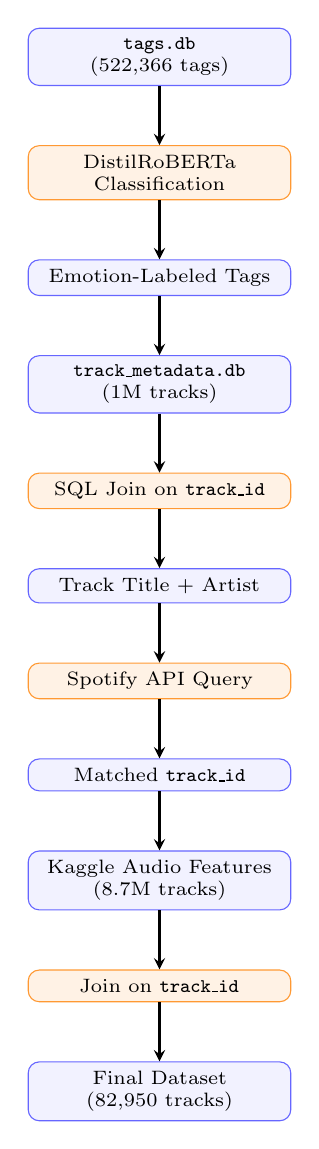
\begin{tikzpicture}[
    node distance=0.75cm,
    every node/.style={font=\scriptsize},
    data/.style={rectangle, draw=blue!60, fill=blue!5, rounded corners, text width=3.1cm, align=center, minimum height=0.8em},
    process/.style={rectangle, draw=orange!80, fill=orange!10, rounded corners, text width=3.1cm, align=center, minimum height=0.8em},
    arrow/.style={->, thick, >=stealth}
]

% Nodes
\node[data] (tagsdb) {\texttt{tags.db}\\(522,366 tags)};
\node[process, below=of tagsdb] (transformer) {DistilRoBERTa Classification};
\node[data, below=of transformer] (robertalabels) {Emotion-Labeled Tags};
\node[data, below=of robertalabels] (trackmeta) {\texttt{track\_metadata.db}\\(1M tracks)};
\node[process, below=of trackmeta] (joinmeta) {SQL Join on \texttt{track\_id}};
\node[data, below=of joinmeta] (trackinfo) {Track Title + Artist};
\node[process, below=of trackinfo] (spotifyquery) {Spotify API Query};
\node[data, below=of spotifyquery] (spotifyid) {Matched \texttt{track\_id}};
\node[data, below=of spotifyid] (kaggledb) {Kaggle Audio Features\\(8.7M tracks)};
\node[process, below=of kaggledb] (joinkaggle) {Join on \texttt{track\_id}};
\node[data, below=of joinkaggle] (finalset) {Final Dataset\\(82,950 tracks)};

% Arrows
\draw[arrow] (tagsdb) -- (transformer);
\draw[arrow] (transformer) -- (robertalabels);
\draw[arrow] (robertalabels) -- (trackmeta);
\draw[arrow] (trackmeta) -- (joinmeta);
\draw[arrow] (joinmeta) -- (trackinfo);
\draw[arrow] (trackinfo) -- (spotifyquery);
\draw[arrow] (spotifyquery) -- (spotifyid);
\draw[arrow] (spotifyid) -- (kaggledb);
\draw[arrow] (kaggledb) -- (joinkaggle);
\draw[arrow] (joinkaggle) -- (finalset);

\end{tikzpicture}
\caption{Emotion labeling and dataset construction pipeline.}
\label{fig:pipeline_final}
\end{figure}



\section{Results}
\subsection{Baseline Model Comparison}

To establish benchmark performance for multi-label music emotion classification, I implemented and evaluated three commonly used classifiers: Multi-Layer Perceptron (MLP), Random Forest, and K-Nearest Neighbors (KNN). All models were trained on the same 12-dimensional audio feature set and evaluated using a top-$k$ dynamic matching strategy, where $k$ corresponds to the number of true labels per instance. This ensures a fairer assessment in the multi-label context and avoids penalizing models for predicting multiple relevant emotions.

\paragraph{Overall Performance.}
Among the three models, \textbf{Random Forest} achieved the highest micro-average F1 score (\textbf{0.6766}) and exact match accuracy (\textbf{36.67\%}). \textit{Exact match accuracy} refers to the proportion of instances for which the predicted emotion set exactly matches the true multilabel set. This is a strict metric in multi-label classification, and a score of 36.67\%, while seemingly modest, is considered relatively strong given the task's complexity and the presence of overlapping emotional labels.

\textbf{MLP} followed closely with an F1 score of 0.6757, benefiting from its ability to capture nonlinear interactions among features. In contrast, \textbf{KNN} underperformed across all metrics, particularly in exact match accuracy (30.30\%) and Hamming Loss (0.2565), likely due to its sensitivity to feature scaling and difficulty modeling sparse multilabel outputs in high-dimensional acoustic space.

\paragraph{Metric Rationale.}
Micro-averaged F1 score was selected as the primary evaluation metric because it accounts for all true positives, false positives, and false negatives across the dataset. Unlike macro F1, which treats all classes equally regardless of frequency, micro F1 provides a more balanced estimate in the presence of class imbalance, which is particularly relevant for music emotion classification where categories like \textit{joy} are overrepresented while \textit{fear} and \textit{disgust} are less common.

Hamming Loss was included to capture the average number of incorrect label assignments per sample. It penalizes both false positives and false negatives uniformly, offering a complementary view of model performance at the label level. A lower Hamming Loss indicates more precise multi-label predictions. In our results, Random Forest produced the lowest Hamming Loss (0.2261), reinforcing its advantage in minimizing unnecessary or missed predictions.

\begin{table}[H]
\centering
\label{tab:model_comparison}
\begin{tabular}{lccccc}
\toprule
\textbf{Model} & \textbf{Micro F1} & \textbf{Exact Match (\%)} & \textbf{Hamming Loss} & \textbf{Macro F1} & \textbf{Weighted F1} \\
\midrule
Random Forest     & \textbf{0.6766} & \textbf{36.67} & \textbf{0.2261} & 0.5379 & 0.6547 \\
MLP               & 0.6757          & 36.27          & 0.2268          & 0.5187 & 0.6436 \\
KNN               & 0.6332          & 30.30          & 0.2565          & 0.5098 & 0.6188 \\
\bottomrule
\caption{Overall performance metrics for three baseline classifiers under top-$k$ dynamic matching.}
\end{tabular}
\end{table}


\paragraph{Per-Class Analysis.}
All models demonstrated strong performance on high-frequency classes such as \textit{joy} and \textit{sadness}, while struggling on low-frequency, ambiguous categories like \textit{fear}, \textit{disgust}, and \textit{surprise}. For instance, as shown in Figure~\ref{fig:per_class_scores}, the Random Forest classifier achieved high F1 scores on \textit{joy} (0.84) and \textit{sadness} (0.76), but much lower scores on \textit{fear} (0.31), \textit{disgust} (0.44), and \textit{surprise} (0.37).

The precision for minority emotions remained relatively stable (around 0.5--0.6), indicating that when the model predicted these emotions, it was often correct. However, the consistently low recall on these categories reveals that the model rarely made such predictions in the first place. For example, \textit{fear} had a recall of only 0.22, while \textit{surprise} was even lower at 0.28. This recall imbalance is a central bottleneck in multilabel music emotion recognition, particularly under weak supervision, and reflects the joint impact of label noise, data imbalance, and subtle or overlapping affective cues.

This asymmetry between precision and recall supports findings in previous literature \parencite{Ahsan2015, Tuba2025}, where minority classes tend to suffer from retrieval failure even when precision is acceptable. These trends motivate the SHAP-based misclassification analysis that follows, which seeks to disentangle how acoustic features—such as valence, tempo, and speechiness—contribute to false negatives under different emotional regimes.

% \begin{figure}[H]
% \centering
% \includegraphics[width=0.8\textwidth]{Graphics/per_class_score/per_class_rf.png}
% \caption{Per-class precision, recall, and F1-score for the Random Forest classifier.}
% \label{fig:per_class_scores}
% \end{figure}
% \FloatBarrier

\subsection{Random Forest Hyperparameter Optimization}

While Random Forest already outperformed other baseline models in its default configuration, additional improvements were achieved through systematic hyperparameter tuning. I conducted a grid search across the following parameter ranges:

\begin{itemize}
    \item \texttt{n\_estimators}: \{100, 200\}
    \item \texttt{max\_depth}: \{None, 10, 20\}
    \item \texttt{min\_samples\_split}: \{2, 5\}
    \item \texttt{min\_samples\_leaf}: \{1, 2\}
\end{itemize}

Using five-fold cross-validation and micro-average F1 as the evaluation metric, the best-performing parameter combination was:

\begin{quote}
\texttt{\{n\_estimators = 200, max\_depth = 20, min\_samples\_split = 2, min\_samples\_leaf = 1\}}
\end{quote}

\paragraph{Performance Gains.}
The optimized Random Forest achieved a micro-average F1 score of \textbf{0.6794}, up from 0.6766 in the baseline. Exact match accuracy rose slightly to \textbf{36.95\%}, and Hamming Loss decreased to \textbf{0.2242}, indicating more precise multilabel predictions. Table~\ref{tab:rf_tuned_performance} summarizes key metrics.

\begin{table}[H]
\centering
\begin{tabular}{|l|c|}
\hline
\textbf{Metric} & \textbf{Score} \\
\hline
Micro Precision & 0.6794 \\
Micro Recall    & 0.6794 \\
Micro F1 Score  & 0.6794 \\
Exact Match Accuracy & 0.3695 \\
Hamming Loss    & 0.2242 \\
\hline
\end{tabular}
\caption{Evaluation metrics for optimized Random Forest model.}
\label{tab:rf_tuned_performance}
\end{table}

\paragraph{Per-Class Improvements.}
The optimized model maintained strong performance on high-frequency classes (\textit{joy}: F1 = 0.83; \textit{sadness}: F1 = 0.75) and modestly improved recognition of rare classes (e.g., \textit{fear}: F1 = 0.28; \textit{surprise}: F1 = 0.35). These F1 scores are computed against transformer-derived emotion labels, which were weakly assigned using a DistilRoBERTa classifier on Last.fm tags. While these labels are not ground truth in the traditional sense, they offer a consistent, semantically meaningful proxy for emotional content across a large-scale music corpus.

Thus, the reported improvements should be interpreted as better alignment with the tag-based semantic emotion mapping pipeline, rather than human-annotated emotional ground truth. Nonetheless, the fact that tuning (e.g., deeper trees, more estimators) helps recover low-frequency emotions more accurately suggests the model is more robust to label sparsity and ambiguity.

These results underscore the importance of careful hyperparameter tuning even for robust ensemble models, particularly when training on large, imbalanced, and noisily labeled datasets.

\subsection{Emotion Label Co-occurrence Patterns}

To better understand the intrinsic structure of the multilabel emotion space, I computed a pairwise co-occurrence matrix over all annotated emotion labels. As shown in Figure~\ref{fig:emotion_cooccur}, several emotion pairs appear frequently together within the same track annotations. For instance, \textit{joy} and \textit{sadness} co-occur in over 15,000 tracks, while \textit{anger} and \textit{disgust} are paired in more than 2,400 instances.

These results confirm that listener-assigned tags often reflect blended or ambivalent affect, consistent with prior observations on low recall for rare classes. The overlap between semantically adjacent categories (e.g., \textit{fear} and \textit{sadness}, \textit{joy} and \textit{surprise}) complicates label separation and contributes to confusion during classification. These patterns further motivate interpretability-driven model diagnostics, presented in the next section.

\begin{figure}[H]
\centering
\includegraphics[width=\textwidth]{Graphics/Emotion_Co_Heatmap.jpg}
\caption{Co-occurrence matrix of emotion labels across multilabel annotations.}
\label{fig:emotion_cooccur}
\end{figure}



\subsection{Global and Per-Label Feature Importance Analysis}

To interpret how each model utilizes acoustic features for multilabel emotion classification, I computed global and per-label feature importance scores across three classifiers: Random Forest (RF), K-Nearest Neighbors (KNN), and Multi-Layer Perceptron (MLP).

\paragraph{Methodology.} To evaluate how models prioritize different audio features, I applied feature importance analysis across three classifier families. For KNN, I used permutation-based importance via a \texttt{OneVsRestClassifier} wrapper and averaged the results across emotion classes. For Random Forest, I extracted built-in \texttt{feature\_importances\_} values from the best estimator. For MLP, I used SHAP’s KernelExplainer on 100 training samples, calculating mean absolute SHAP values for each feature and averaging them globally and per emotion class.

\begin{figure}[H]
\centering
\includegraphics[width=0.85\textwidth]{Graphics/global_feature_importance_comparison.png}
\caption{Global feature importance scores across models. MLP importance computed via SHAP; Random Forest and KNN via permutation.}
\label{fig:feature_importance}
\end{figure}

As shown in Figure~\ref{fig:feature_importance}, Random Forest emphasized \texttt{acousticness}, \texttt{loudness}, and \texttt{energy}—features with sharp thresholds well-suited to tree-based decision boundaries. The high importance of \texttt{acousticness} (0.1214) aligns with its role in differentiating unplugged and high-arousal music, consistent with prior affective MIR findings \parencite{Huron2015, McCraty1998}.

KNN placed more weight on \texttt{danceability}, \texttt{valence}, and \texttt{mode}, suggesting that similarity-based classification is more influenced by rhythmic and tonal characteristics—features that likely produce tighter clusters in Euclidean space.

MLP showed more balanced attribution across features, reflecting its ability to capture nonlinear combinations. SHAP results indicated \texttt{speechiness}, \texttt{energy}, and \texttt{acousticness} as particularly influential. These dimensions may encode expressive subtleties (e.g., rap-like vocals or whispered tones) that are difficult for tree-based or distance-based models to capture.

Across all models, \texttt{key}, \texttt{mode}, and \texttt{time\_signature} consistently received low importance scores—consistent with the weak correlation patterns observed earlier. These features likely offer marginal predictive power in large, genre-diverse datasets and may matter only in niche musical contexts.

To examine model behavior at the emotion-specific level, I visualized SHAP-derived feature importances for each emotion class using the MLP classifier (Figures~\ref{fig:shap_anger} to~\ref{fig:shap_surprise}). While \texttt{energy} and \texttt{loudness} remained influential across most categories, distinct feature-emotion associations emerged:

\paragraph{Anger.} Driven by \texttt{speechiness} and \texttt{acousticness}, potentially reflecting intense or shouted vocal styles.

\begin{figure}[H]
\centering
\includegraphics[width=0.8\linewidth]{Graphics/per_label/anger_feature_importance.png}
\caption{Feature importance (MLP SHAP) for emotion: \textit{anger}}
\label{fig:shap_anger}
\end{figure}

\paragraph{Disgust.} Emphasizes \texttt{instrumentalness} and \texttt{liveness}, indicating textural or ambient styles with minimal lyrics.

\begin{figure}[H]
\centering
\includegraphics[width=0.8\linewidth]{Graphics/per_label/disgust_feature_importance.png}
\caption{Feature importance (MLP SHAP) for emotion: \textit{disgust}}
\label{fig:shap_disgust}
\end{figure}

\paragraph{Fear.} Relies on \texttt{valence} and \texttt{energy}, consistent with literature on low-valence, high-arousal fear profiles.

\begin{figure}[H]
\centering
\includegraphics[width=0.8\linewidth]{Graphics/per_label/fear_feature_importance.png}
\caption{Feature importance (MLP SHAP) for emotion: \textit{fear}}
\label{fig:shap_fear}
\end{figure}

\paragraph{Joy.} Strong influence from \texttt{speechiness}, aligning with rhythmic, lyric-heavy delivery.

\begin{figure}[H]
\centering
\includegraphics[width=0.8\linewidth]{Graphics/per_label/joy_feature_importance.png}
\caption{Feature importance (MLP SHAP) for emotion: \textit{joy}}
\label{fig:shap_joy}
\end{figure}

\paragraph{Sadness.} Elevated \texttt{acousticness} and reduced \texttt{loudness}, capturing softer, more introspective tones.

\begin{figure}[H]
\centering
\includegraphics[width=0.8\linewidth]{Graphics/per_label/sadness_feature_importance.png}
\caption{Feature importance (MLP SHAP) for emotion: \textit{sadness}}
\label{fig:shap_sadness}
\end{figure}

\paragraph{Surprise.} Prioritizes \texttt{liveness}, \texttt{tempo}, and \texttt{energy}, likely reflecting unexpected or high-intensity dynamics.

\begin{figure}[H]
\centering
\includegraphics[width=0.8\linewidth]{Graphics/per_label/surprise_feature_importance.png}
\caption{Feature importance (MLP SHAP) for emotion: \textit{surprise}}
\label{fig:shap_surprise}
\end{figure}


Together, these findings reinforce the value of per-label interpretation in multi-label settings. They demonstrate that while some features are broadly predictive, others contribute selectively, depending on the emotional context. This justifies the subsequent ablation and correlation-based redundancy analyses.

\subsection{Feature Correlation Analysis}

To assess potential collinearity among audio features, I computed the Pearson correlation matrix and visualized it as a heatmap. This analysis helps identify redundant predictors and informs downstream decisions on feature selection, normalization, and model interpretation.

Several noteworthy patterns emerged. The strongest negative correlations appear between \texttt{acousticness} and \texttt{energy} ($r = -0.72$), as well as \texttt{acousticness} and \texttt{loudness} ($r = -0.58$), indicating that acoustic tracks tend to be quieter and less energetic. Conversely, \texttt{energy} and \texttt{loudness} show a strong positive correlation ($r = 0.76$), aligning with perceptual theories linking amplitude to arousal. \texttt{Danceability} moderately correlates with \texttt{valence} ($r = 0.55$), suggesting that rhythmically engaging tracks are more likely to be perceived as emotionally positive.

In contrast, features such as \texttt{key}, \texttt{mode}, and \texttt{time\_signature} exhibit weak or near-zero correlations with other variables. This suggests minimal linear interaction and implies that their potential emotional influence may arise only through nonlinear or genre-specific mechanisms.

\begin{figure}[H]
\centering
\includegraphics[width=\textwidth]{Graphics/feature_correlation.png}
\caption{Pearson correlation matrix of the 12 Spotify audio features.}
\label{fig:feature_correlation}
\end{figure}

These findings underscore the rationale for incorporating permutation-based and SHAP-based importance methods in the modeling pipeline, as they capture model-relevant feature contributions beyond linear correlation.

\subsection{Ablation Study}

To examine feature redundancy and the robustness of model performance, I conducted a stepwise ablation study. Features were removed in ascending order of global importance (as determined by Random Forest importance scores), and the model was retrained and evaluated at each step using the same multilabel dynamic top-$k$ strategy.

\begin{table}[H]
\centering
\resizebox{\textwidth}{!}{
\begin{tabular}{|c|c|l|}
\hline
\textbf{Remaining Features} & \textbf{Accuracy} & \textbf{Dropped Features} \\
\hline
12 & 0.2403 & [] \\
11 & 0.2361 & [valence] \\
10 & 0.2361 & [valence, loudness] \\
9  & 0.2182 & [valence, loudness, instrumentalness] \\
8  & 0.2069 & [valence, loudness, instrumentalness, energy] \\
7  & 0.1904 & [valence, loudness, instrumentalness, energy, acousticness] \\
6  & 0.1890 & [valence, loudness, instrumentalness, energy, acousticness, danceability] \\
5  & 0.1932 & [valence, loudness, instrumentalness, energy, acousticness, danceability, speechiness] \\
4  & 0.1767 & [valence, loudness, instrumentalness, energy, acousticness, danceability, speechiness, liveness] \\
3  & 0.2201 & [\dots, tempo] \\
2  & 0.2347 & [\dots, key] \\
1  & 0.2370 & [\dots, mode] \\
\hline
\end{tabular}
}
\caption{Ablation study: effect of sequential feature removal on prediction accuracy. Features removed in ascending order of importance.}
\label{tab:ablation_study}
\end{table}

\begin{figure}[H]
\centering
\includegraphics[width=0.75\textwidth]{Graphics/Ablation Study.png}
\caption{Ablation study: Random Forest accuracy as a function of remaining features. Features are removed in ascending order of global importance.}
\label{fig:ablation_study}
\end{figure}

As shown in Figure~\ref{fig:ablation_study}, model accuracy declined most significantly after removing the top five features—\texttt{acousticness}, \texttt{energy}, \texttt{loudness}, \texttt{valence}, and \texttt{instrumentalness}—dropping to 0.1767 when only four features remained. This confirms that a concentrated subset of acoustic features carries most of the predictive signal for emotional classification.

Interestingly, accuracy partially rebounded as more low-importance features were excluded. Removing variables such as \texttt{key}, \texttt{mode}, and \texttt{time\_signature} appeared to reduce noise rather than degrade performance. This observation is consistent with earlier findings in both the correlation analysis and global importance scores, where these features showed weak or inconsistent contributions.

To explore the impact of dimensionality reduction, I also tested the best-performing model without applying PCA. Results improved modestly: Micro-F1 rose to 0.690 and Exact Match Accuracy increased to 0.388. Notably, precision for rare labels like \textit{disgust} and \textit{fear} rose to 0.57 each, suggesting that preserving full dimensionality may enhance detection of subtle patterns that PCA might otherwise suppress.

Overall, the ablation analysis reinforces earlier interpretations: emotion classification is driven by a compact set of expressive acoustic features, while categorical or low-variance metadata often offer limited marginal value and can be safely excluded.

\subsection{Per-Class Metrics and Shared Errors}

As shown in Figure~\ref{fig:per_class_scores}, precision, recall, and F1-score vary widely across emotional categories. \textit{Joy} and \textit{Sadness} are predicted with high accuracy (F1 = 0.83 and 0.75, respectively), while \textit{Fear}, \textit{Surprise}, and \textit{Disgust} perform poorly (F1 = 0.28–0.42), driven largely by low recall.

The misclassification heatmap in Figure~\ref{fig:confusion_heatmap} reveals systematic confusion patterns. \textit{Sadness} is often misclassified as \textit{Joy} (53\%), and \textit{Fear} as either \textit{Sadness} or \textit{Joy}. These errors reflect both co-occurrence tendencies and overlapping acoustic signals between emotional categories.

\begin{figure}[H]
\centering
\includegraphics[width=0.6\textwidth]{Graphics/Error Analysis/True to Wrongly Predicted.png}
\caption{Heatmap showing frequent misclassification pathways (True → Predicted).}
\label{fig:confusion_heatmap}
\end{figure}

\subsection{Impact of Emotion Co-occurrence}

To examine whether co-occurring emotion labels affect misclassification, I computed the average number of co-labels per instance when each emotion is present and plotted it against false negative rates (Figure~\ref{fig:cooccur_missrate}). A clear inverse relationship emerges: emotions with more frequent co-occurrence—such as \textit{Surprise} and \textit{Fear}—are more likely to be missed entirely. In contrast, \textit{Joy} is rarely missed, likely due to its distinctive acoustic profile.

This negative correlation suggests that emotion categories with higher co-labeling rates tend to be more context-dependent, reducing model confidence in isolating them during prediction.

\begin{figure}[H]
\centering
\includegraphics[width=0.6\textwidth]{Graphics/Error Analysis/Emotion Co vs Missed Prediction Rate.png}
\caption{Relationship between average emotion co-occurrence and prediction miss rate.}
\label{fig:cooccur_missrate}
\end{figure}

\subsection{SHAP-Based Interpretation of Misclassified Samples}

To probe why certain emotions are more difficult to classify, I conducted SHAP-based interpretation on one misclassified example per emotion. All predictions were thresholded based on dynamic top-$k$ label matching; hence, scores below a track’s $k$-ranked threshold were excluded from final outputs. Each SHAP waterfall plot visualizes how individual feature values contributed to the model’s final decision.

\textbf{Anger}: The model predicted a confidence score of 0.583 but still fell short of the top-$k$ cutoff. High \texttt{energy} and low \texttt{valence} were positively associated with anger—consistent with aggressive delivery and negative emotional tone. However, low \texttt{tempo} and abnormal \texttt{time\_signature} contributed negatively, suggesting rhythmic ambiguity may mask anger cues.

\begin{figure}[H]
\centering
\includegraphics[width=0.55\textwidth]{Graphics/shap_missed_labels/anger_missed_shap_waterfall.png}
\caption{SHAP explanation for misclassified \textit{Anger}.}
\label{fig:shap_anger}
\end{figure}

\textbf{Disgust}: Moderate \texttt{speechiness}, \texttt{energy}, and low \texttt{valence} were aligned with disgust, but weak contributions from \texttt{loudness} and \texttt{danceability}, and negative influence from \texttt{instrumentalness}, indicate that disgust lacks consistent acoustic signatures.

\begin{figure}[H]
\centering
\includegraphics[width=0.55\textwidth]{Graphics/shap_missed_labels/disgust_missed_shap_waterfall.png}
\caption{SHAP explanation for misclassified \textit{Disgust}.}
\label{fig:shap_disgust}
\end{figure}

\textbf{Fear}: This sample showed the lowest model confidence (0.124). Features such as high \texttt{speechiness} and low \texttt{energy} had contradictory impacts, effectively canceling each other out. The model failed to find a dominant signal—nearly all contributions were near zero.

\begin{figure}[H]
\centering
\includegraphics[width=0.55\textwidth]{Graphics/shap_missed_labels/fear_missed_shap_waterfall.png}
\caption{SHAP explanation for misclassified \textit{Fear}.}
\label{fig:shap_fear}
\end{figure}

\textbf{Joy}: Although high in \texttt{energy}, \texttt{danceability}, and \texttt{acousticness}, the prediction fell short due to low \texttt{speechiness} and \texttt{tempo}. This highlights the importance of rhythmic and lyrical expressiveness in joyful tracks.

\begin{figure}[H]
\centering
\includegraphics[width=0.55\textwidth]{Graphics/shap_missed_labels/joy_missed_shap_waterfall.png}
\caption{SHAP explanation for misclassified \textit{Joy}.}
\label{fig:shap_joy}
\end{figure}

\textbf{Sadness}: Surprisingly, low \texttt{tempo} and \texttt{energy} pushed the score downward. Although expected to correlate with sadness, the model may rely more heavily on \texttt{acousticness} or \texttt{instrumentalness}, which were absent in this case.

\begin{figure}[H]
\centering
\includegraphics[width=0.55\textwidth]{Graphics/shap_missed_labels/sadness_missed_shap_waterfall.png}
\caption{SHAP explanation for misclassified \textit{Sadness}.}
\label{fig:shap_sadness}
\end{figure}

\textbf{Surprise}: Despite moderate \texttt{loudness}, \texttt{mode}, and \texttt{danceability}, high \texttt{acousticness} suppressed the prediction. This suggests the model interpreted the track as introspective rather than surprising, highlighting ambiguity in acoustic cues.

\begin{figure}[H]
\centering
\includegraphics[width=0.55\textwidth]{Graphics/shap_missed_labels/surprise_missed_shap_waterfall.png}
\caption{SHAP explanation for misclassified \textit{Surprise}.}
\label{fig:shap_surprise}
\end{figure}

\begin{table}[H]
\centering
\begin{tabular}{|l|l|p{8.5cm}|}
\hline
\textbf{Failure Mode} & \textbf{Emotion} & \textbf{Explanation} \\
\hline
Overlapping semantics & Sadness $\rightarrow$ Joy & Bittersweet or nostalgic tone interpreted as positive due to instrumentation \\
Lack of dominant cues & Fear & Weak signal across all features, leading to model indecision \\
Feature conflict & Disgust & Noisy combination of low valence but ambiguous rhythmic/timbral signals \\
Rhythmic mismatch & Anger, Joy & Tempo and time signature inconsistent with model prototype of class \\
Cultural encoding & Surprise & Subtle emotional valence varies by genre; high acousticness misinterpreted \\
\hline
\end{tabular}
\caption{Typology of common failure modes in multilabel music emotion classification.}
\label{tab:failure_typology}
\end{table}


\section{Discussion}

This study set out to investigate how supervised machine learning models interpret Spotify-derived acoustic features when classifying songs into emotional categories under a weakly supervised, multilabel framework. Rather than focusing solely on model performance metrics, the analysis prioritized interpretability—both in terms of which features drive predictions and how failure cases reveal the limits of audio-based emotion modeling.

The error analysis reveals that model performance is unevenly distributed across emotion categories. Emotions like 	extit{joy} and 	extit{sadness} exhibit strong precision and recall, whereas 	extit{fear}, 	extit{disgust}, and 	extit{surprise} remain highly error-prone. The confusion heatmap and co-occurrence diagnostics suggest that many prediction failures arise not from model incapacity, but from the inherent fuzziness of emotional boundaries and frequent label overlap. For example, 	extit{fear} was often confused with both 	extit{sadness} and 	extit{joy}, indicating ambiguity in acoustic and affective space. This observation is further supported by the inverse correlation between co-occurrence frequency and false negative rate: emotions that frequently co-appear (e.g., 	extit{fear}, 	extit{surprise}) tend to be missed more often due to weaker standalone signal and context dependence.

SHAP-based misclassification analysis further supports this observation. In most misclassified samples, no single feature was strongly misleading; rather, the predictions were undermined by diffuse, low-magnitude signals or contradictory cues across features. This “absence of dominant signal” failure mode was particularly evident in 	extit{fear}, where near-zero SHAP values across all features resulted in model indecision. These errors are thus not classic misclassifications, but reflections of semantic ambiguity—a finding consistent with prior work on weakly supervised emotional tags \parencite{Artemova2025, Kim2024}.

Global feature importance scores and SHAP-based interpretation confirm that high-variance, perceptually salient features play a dominant role in emotional inference. Features like \texttt{energy} and \texttt{valence} map closely to psychological models of arousal and positivity \parencite{Huron2015, McCraty1998}, while high \texttt{acousticness} was particularly diagnostic for sadness and fear. However, models diverged in how they leveraged these cues: MLP distributed importance more evenly across the feature space and captured subtle nonlinear interactions, while KNN relied heavily on cluster-inducing features such as \texttt{danceability} and \texttt{mode}, reflecting its sensitivity to local neighborhood structure.

While Random Forest achieved the highest micro-average F1 score and exact match accuracy, this outcome should be interpreted with caution. RF requires less extensive hyperparameter tuning and was the only model in this study subjected to full grid search optimization. As such, its performance advantage may partially reflect tuning effort rather than inherent model superiority.

The ablation study further revealed that emotional classification is driven by a compact yet semantically rich acoustic subspace. Removing the top five features led to a 26% drop in accuracy. Interestingly, performance partially rebounded when weakly informative features (e.g., \texttt{key}, \texttt{mode}, \texttt{time_signature}) were removed. This suggests that including noise-prone or low-variance features may reduce model robustness—despite their theoretical relevance in tonal analysis. Feature correlation analysis also confirms this: \texttt{energy} and \texttt{loudness} were highly correlated, but not fully redundant, since both contributed unique nonlinear interactions in certain emotion classes.

SHAP-based local analyses also identified common failure typologies. For example, misclassified samples of \textit{disgust} showed low valence and moderate speechiness but lacked rhythmic or timbral cues to anchor the classification. Similarly, surprise was often misinterpreted as introspective or melancholic when acousticness was high, suggesting a failure to capture cultural or genre-specific emotional conventions—particularly in jazz or swing, where surprise is embedded more in performance dynamics than in raw audio features.

The study also finds that label ambiguity and emotional co-occurrence remain significant challenges. As the emotion co-occurrence vs. miss rate analysis shows, labels that frequently co-occur with others—such as \textit{fear} and \textit{surprise}—are more likely to be missed entirely. This aligns with prior research showing that label overlap and fuzzy category boundaries are common in affective annotation, especially when based on crowd-generated or inferred labels \parencite{Kim2024, Yang2024}. Top-$k$ prediction thresholds also compound this issue, as predictions just below cutoff—while semantically valid—are excluded from evaluation.

Manual inspection of misclassified examples further complicates the interpretation of "error." For instance, Billie Holiday’s \textit{All of Me} was labeled with anger, sadness, and joy, but the model predicted only joy. This outcome, while technically incorrect, is arguably a valid representation of the song’s musical tone. Such cases underscore the distinction between algorithmic misclassification and perceptual disagreement, and raise questions about the epistemological status of crowd-sourced ground truth.

From a methodological perspective, this study demonstrates the value of integrating SHAP analysis, co-occurrence diagnostics, and ablation studies to interpret not just what the model predicts but how and why. While permutation-based feature importance offered a reliable global overview, SHAP waterfall plots revealed feature interactions and borderline cases that would have otherwise been overlooked. The joint use of global and local attribution methods proved especially helpful in mapping failure modes and guiding model refinement.

\subsection{Limitations}

Despite its contributions, this study has several limitations related to the labeling pipeline, data matching, feature design, interpretability analysis, and evaluation strategy.

The most fundamental limitation lies in the use of automatically generated emotion labels rather than human-annotated ground truth. Labels were derived from a DistilRoBERTa classifier applied to Last.fm user tags, which are often genre-centric, polysemous, or aesthetically focused (e.g., \textit{lo-fi}, \textit{dream pop}) rather than affective in nature. While transformer models have shown promise in extracting sentiment from sparse or ambiguous text \parencite{Kim2024, Artemova2025}, their performance on style-tagged musical metadata remains insufficiently validated. As a result, this introduces the risk of semantic misalignment, where the labeler might systematically infer emotion categories that diverge from listener intent. Moreover, using these same labels to train and evaluate classifiers risks a form of circular validation: models are tested against the outputs of another model with similar representational assumptions. This reduces the trustworthiness of performance metrics and makes it difficult to assess generalization.

The reliance on a dynamic top-K threshold for multilabel prediction introduces another layer of abstraction. Although this strategy respects label cardinality and improves macro accuracy, it still imposes a hard cutoff that may exclude borderline but semantically valid predictions. This is especially problematic for ambiguous emotions like \textit{surprise} and \textit{fear}, which tend to co-occur with other emotions and are thus often pushed below the decision threshold. As a result, recall suffers disproportionately for less dominant classes, even when model confidence is moderate.

The expressiveness of the emotion taxonomy is also limited. The six fixed emotion categories used—while aligned with basic emotion theory—do not capture the full complexity of musical affect. Emotions in music often blend, evolve over time, or defy discrete classification altogether. Models trained on fixed labels may struggle with such gradations or with culturally specific emotion encodings. Incorporating soft label distributions or continuous valence-arousal modeling may offer more fidelity in future work.

A further limitation concerns the confidence threshold used during emotion label generation. To focus on affect-rich tags and reduce ambiguity, the pipeline retained only emotion predictions with a model-assigned confidence score above 0.8 and excluded neutral outputs. While this strategy helps ensure semantic clarity—e.g., the tag \textit{happy} was mapped to \textit{joy} with 0.993 confidence—it also introduces an arbitrary hyperparameter without systematic justification. The decision to use a 0.8 cutoff, rather than 0.75 or 0.85, was not empirically tuned. Without testing the robustness of downstream results across different thresholds, it remains unclear whether key findings depend critically on this design choice. Future work should rerun the full pipeline across a range of thresholds to evaluate sensitivity and ensure that observed patterns are not artifacts of a single filtering criterion.

Coverage is further constrained by metadata matching. Due to API limitations, misspellings, and missing metadata in the Million Song Dataset, a nontrivial subset of Last.fm tracks could not be matched to Spotify IDs. Furthermore, a portion of matched tracks lacked complete Spotify audio features, reducing the final sample to a filtered subset of 82,950 rows. These constraints likely bias the dataset toward more mainstream, Western, and well-indexed music, limiting generalizability to underrepresented genres or regions.

The audio representation itself poses further limitations. Although Spotify’s 12-dimensional feature set captures coarse-grained acoustic properties (e.g., \texttt{energy}, \texttt{valence}, \texttt{danceability}), it excludes temporal dynamics, harmonic progression, lyrical sentiment, and melodic arcs—all of which are known to influence affective judgment. For instance, a slow tempo may suggest sadness in classical music but tension in post-rock. Without incorporating these higher-order features, the model may over-rely on surface-level cues that lack genre specificity.

Interpretability tools used in this study also have technical caveats. The SHAP KernelExplainer applied to MLP models requires extensive computation and is limited to small reference sets (e.g., 100 samples), potentially reducing the statistical robustness of per-label explanations. Moreover, SHAP is sensitive to feature collinearity: in highly correlated contexts (e.g., \texttt{loudness} and \texttt{energy}), importance may be arbitrarily split or suppressed. For Random Forests, axis-aligned splits may favor some features simply because they happen to create clearer thresholds. These artifacts complicate model comparison across architecture families and reduce the interpretive fidelity of local explanations.

Although dimensionality reduction (e.g., PCA) was initially considered, it was ultimately omitted to preserve interpretability. While this decision helped amplify weak signals for minority labels like \textit{disgust}, it may have also retained redundant or noisy features that hurt model clarity or generalization. Future work could benefit from SHAP-guided pruning or domain-aware selection strategies that reduce noise while preserving semantic diversity.

The evaluation strategy is further limited by its reliance on $\hat{y}$ as ground truth. Because many songs are labeled with only a subset of their possible emotions, and because tagging behaviors vary across genres and communities, some correct predictions may be penalized as false positives. This makes standard metrics like F1 and Exact Match Accuracy less informative in the presence of labeling incompleteness, especially for emotions with low coverage or high contextual ambiguity.

Lastly, cultural and genre-based biases embedded in both the training tags and model inferences pose significant challenges. Some genres (e.g., jazz, ambient, experimental) may convey emotion through non-lexical cues like performance practice, instrumentation, or tempo variation, which fall outside the representational range of current feature sets. For example, \texttt{acousticness} may be interpreted as melancholic in folk but as upbeat or playful in swing. The current pipeline is not equipped to resolve these cross-cultural or intra-genre shifts, which limits its interpretability and fairness across musical traditions.

To address these limitations, future research should integrate human-coded annotations to benchmark weakly supervised labels, incorporate multimodal features such as lyrics, melodic embeddings, or genre metadata, and apply robust, scalable interpretability frameworks. More diverse and context-aware datasets—spanning languages, styles, and listener populations—will also be critical for building emotion classifiers that generalize meaningfully across musical cultures.



\section{Conclusion}

This study investigated the capacity of supervised machine learning models to classify the emotional character of songs using only Spotify-derived acoustic features. Leveraging a weakly supervised labeling pipeline, where emotion labels were generated from Last.fm tags via a DistilRoBERTa transformer, the final dataset enabled multilabel classification across six basic emotions: anger, disgust, fear, joy, sadness, and surprise.

Among the three models evaluated—Random Forest, K-Nearest Neighbors, and Multi-Layer Perceptron—Random Forest achieved the best overall performance in micro F1 score and exact match accuracy. Its robustness stemmed from its ability to isolate thresholdable acoustic features such as \texttt{acousticness}, \texttt{energy}, and \texttt{loudness}. However, prediction accuracy varied substantially across classes: \textit{joy} and \textit{sadness} were modeled with high confidence, while \textit{fear}, \textit{disgust}, and \textit{surprise} remained challenging due to lower feature salience, frequent co-occurrence, and emotional ambiguity. These performance asymmetries highlight the difficulty of disambiguating nuanced emotional states from audio alone, especially in the absence of temporal or lyrical context.

Interpretability played a central role in this study. Global feature importance comparisons revealed model-specific preferences for acoustic cues: tree-based models prioritized variance and separability; MLPs captured non-linear interactions; KNN emphasized cluster geometry in the feature space. SHAP-based local explanations revealed that many classification failures were not due to noisy input but instead reflected semantically ambiguous acoustic profiles or weak feature interactions—underscoring the fuzzy boundaries between affective categories.

An ablation study reinforced the centrality of a compact emotional subspace. Removal of top-ranked features such as \texttt{acousticness}, \texttt{energy}, and \texttt{valence} led to a substantial drop in accuracy, confirming their foundational role in affective inference. However, the study also surfaced critical limitations. Emotion labels were inferred, not empirically validated; transformer predictions may be systematically biased by genre conventions or semantic ambiguity in tags. Additionally, the use of top-$k$ label thresholding, while beneficial for precision, introduced recall trade-offs—especially for minority or co-occurring labels like \textit{fear} and \textit{surprise}. These design choices constrained the expressiveness of the output and suppressed emotional plurality.

The generalizability of findings is further limited by dataset coverage. Metadata mismatches and API failures excluded a nontrivial subset of tracks, skewing the corpus toward Western or well-indexed music. Furthermore, the fixed Spotify feature set omits higher-order musical structure, lyrical meaning, and cultural framing, all of which are essential to fully capture affective nuance. SHAP interpretability, while useful, was also constrained by sample size and sensitivity to model architecture—limiting cross-model comparison.

Taken together, this study demonstrates that acoustic features can provide a meaningful foundation for emotion recognition in music, but they are insufficient on their own. Accurate, psychologically plausible modeling of musical affect requires a richer input space and more nuanced evaluative frameworks. Future work should incorporate lyrical content, melodic and harmonic progression, and listener-reported emotion ratings. Labeling pipelines should be benchmarked against human-coded subsets and adapted to support fuzzy or probabilistic emotion targets. Moreover, cross-cultural and genre-aware design will be necessary to ensure models generalize beyond the aesthetics of dominant musical traditions.

In sum, while supervised models can learn valuable emotional patterns from Spotify audio features, achieving true emotional fidelity requires moving beyond the acoustic surface toward a multimodal, human-centered understanding of music’s affective power.


\newpage
\printbibliography

\newpage

\appendix
\section*{Appendix}
\addcontentsline{toc}{section}{Appendix}

\subsection*{Per-Class Performance by Model}
\label{app:per_class_metrics}

\paragraph{K-Nearest Neighbors (KNN).}
As shown in Figure~\ref{fig:per_class_knn}, KNN achieved high recall and F1-score for \textit{joy} and \textit{sadness} (recall = 0.87, 0.80), but struggled significantly on low-frequency emotions such as \textit{fear} and \textit{disgust}, with F1-scores below 0.40. The overall precision remained moderate, but the poor recall for minority classes underscores the difficulty of using distance-based classifiers under class imbalance and high-dimensional feature noise.

\begin{figure}[H]
\centering
\includegraphics[width=0.8\textwidth]{Graphics/per_class_score/per_class_knn.png}
\caption{Per-class metrics for K-Nearest Neighbors classifier.}
\label{fig:per_class_knn}
\end{figure}


\paragraph{Multi-Layer Perceptron (MLP).}
Figure~\ref{fig:per_class_mlp} reveals that the MLP shows better balance between precision and recall. However, the recall for \textit{fear} and \textit{surprise} remained low (0.18 and 0.22 respectively), suggesting that even non-linear models with sufficient capacity struggle when emotion signals are weak or overlapping.

\begin{figure}[H]
\centering
\includegraphics[width=0.8\textwidth]{Graphics/per_class_score/per_class_mlp.png}
\caption{Per-class metrics for Multi-Layer Perceptron classifier.}
\label{fig:per_class_mlp}
\end{figure}



\end{document}
